\documentclass{myproc}
%\addtolength{\topmargin}{-2cm}
%\addtolength{\textheight}{2cm}
\usepackage{mathptm,mydef}
\usepackage{graphicx}
\DeclareGraphicsExtensions{.png,.jpg}
%\usepackage{courier}
\usepackage{epsfig}
\usepackage{alltt}
\usepackage[T1]{fontenc}
%\renewcommand{\ttdefault}{txtt}
\usepackage[all]{xy}
%\usepackage{MinionPro}

\usepackage{hyperref}
\hypersetup{
    colorlinks, 
    citecolor=black, 
    filecolor=black, 
    linkcolor=blue, 
    urlcolor=black
}

\begin{document}
\small


\begin{center}
{\large\bf Google Nest: Overview}
\end{center}

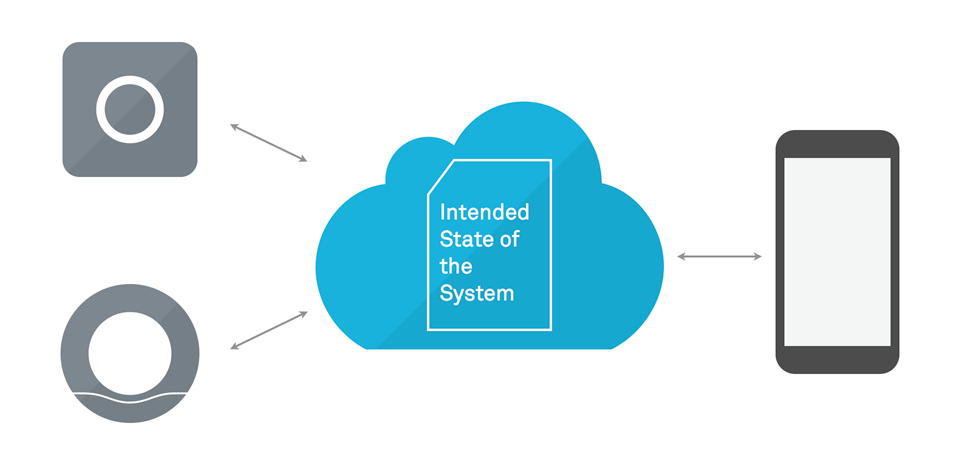
\includegraphics[width=8cm]{pics/intended-state}

\vspace*{1cm}

\tableofcontents

%\pagebreak

\section{Introduction}
\subsection{High-level summary}
\bit
\w \textcolor{red2}{\bf Nest applications allow users to connect with their
  home from wherever they may be.} 
\w There are three components:
  \bit
  \w \bb{Nest devices:} Learning Thermostat, Smoke + CO Alarm, Home (will
  grow as more manufactures adopt Nest)
       \bit
       \w \bb{thermostat}: get/set temperature, set fan timer, get/set mode,
       get online-status/last-connection
       \w \bb{smoke+CO alarm}: get CO/smoke status, get battery helath, get online-stat/last-connection
       \w \bb{home}: get devlice list, get energy event, set \bb{ETA}, get/set
       \bb{Away} state 
       \eit
  \w \bb{Applications:} iOS, Android, web apps
  \w \bb{Nest service}: \textcolor{red2}{\bf Intended State of the System} --
  some ``persistent DB'' in JSON format
      \bit
      \w provides a \bb{data model} of the home
      \w ``devices'' and ``applications'' read from this data model to take
      appropriate actions; write to the data model
      \w \textcolor{blue2}{it's very likely that this is just some pub-sub
        protocol layer}
      \eit
  \eit 
\eit
\subsection{Using Nest API}
\bit
\w register for Nest Developer program
\w build with Firebase client libraries
\w test with Nest developer chrome extension
\eit

\subsection{Firebase client libraries}
\bit
\w Web, iOS, Android
\w allows to synchronize data with a subscription-based 
    near-real time platform
\w Firebase Data Structure
\w API for reading/writing data from \bb{data model}
\eit

\subsection{Data model}
The ``Home'' which contains {\em Nest devices\/} maintains some sort of
persistent data (just like DB) in the form of JSON document.
There are a few defined ``DB tables'' -- \textcolor{blue2}{\bf{}Structures}
and \textcolor{blue2}{\bf{}Thermostats}.

\section{Architecture}
\bit
\w \textcolor{red2}{\bf{}Nest devices operate in highly constrained
  environments.}
   \bit
   \w  power is limited
   \w connectivity is unreliable
   \eit
\eit

\subsection{Firebase}
\bit
\w provides a \bb{real-time data synchronization service}, with intuitive
clients on a broad range of platforms. Rather than build our own clients,
we've instead implemented their service protocols. This means Nest developers
can use Firebase's clients to interact with homes and devices. 
\w provides a \bb{high-level API} for real time data synchronization. With
these libraries, developers can create a responsive, robust client integration
without having to spend as much time worrying about network programming. 
\w \textcolor{blue2}{\bf{}Looks like a very simple ``active database'', where
  the data is stored as JSON document}
\eit


\subsection{Data model}
\bit
\w Your clients will communicate with structures and devices via a shared
\bb{JSON document stored in the service\/} -- i.e. \textcolor{red2}{\bf{}a persistent DB is maintained in the form
     of a JSON document}
\w Data in this document is organized hierarchically. At the top level we have
devices and structures. Specific device types are modeled under the devices
object. 
\w \textcolor{red2}{\bf{}Clients can read and write sections of this document, and
  can also {\em subscribe} to changes in sections of the document.} 
    \bit
    \w This subscription capability allows clients to react in real time to
    changes made to the system, for example, turning off lights when a user
    sets the structure to away. 
    \eit
\begin{alltt}
  \{
    "devices": \{
      "thermostats": \{
        "peyiJNoTldAksjfAKQ": \{
        \}
      \},
      "smoke_co_alarms": \{
        "RTMSkdfjaskAskdjfQAskdjfS": \{
        \}
      \}
    \},
    "structures": \{
        "Vqdj439sAjfjk00askAS": \{
        \}
    \}
  \}
\end{alltt}
\eit

\subsection{Structures object}
\subsubsection{Data values}
\bit
\w \bb{Name}: The name of the structure defaults to \textcolor{red2}{\bf{}''Home''}
\w \bb{Metadata}:  All data values are read only, unless otherwise specified.
   \bit
   \w \textcolor{red2}{\texttt{structure\_id}}: a string that uniquely represents this structure, every developer will see a different ID for the same structure, but multiple clients from the same developer will see the same ID
   \w \textcolor{red2}{\texttt{country\_code}}: an ISO 3166-1 alpha-2 country code that maps to the registered location of the structure
   \w \textcolor{red2}{\texttt{time\_zone}}:  an IANA time zone string that
   maps to the structure's time zone
   \eit

\w \bb{Devices}: Nest devices are listed by type as an array of IDs, which can
be used to uniquely identify a device via the device path. So a thermostat ID
of \textcolor{red2}{\texttt{peyiJNo0IldT2YlIVtYaGQ}} means you could load the thermostats device model at
\textcolor{red2}{\texttt{/devices/thermostats/peyiJNo0IldT2YlIVtYaGQ}} via the Firebase API. The same
would apply to smoke and CO alarms.

\w \bb{Away}:
Access to this field requires Away read or Away read/write permission.
With the Away read permission you can see if Nest thinks the structure is occupied. The possible states are:
  \bit
  \w \textcolor{red2}{\texttt{home}}: there is someone in the house, either because Nest has high confidence from motion sensor data, or the user has explicitly set the structure to home via a Nest App, your client, or via ETA.
  \w  \textcolor{red2}{\texttt{away}}: the user has explicitly set the structure to away, either via a Nest App or your client.
  \w \textcolor{red2}{\texttt{auto-away}}: Nest has determined algorithmically
  that no one is home. Currently there is no way to vote on entering this
  state via the Nest API. Clients are expected to use explicit controls or
  actions that will set away directly rather than algorithmically.
  \eit
Be aware that there are only two ways to change the state from away to home:
   \bit
   \w manually, when the user actively selects it
   \w algorithmically, via ETA
   \eit
Conversely, the only way to change state from home to away is manually.
\w \bb{Energy programs}:
  If a user has paired their Nest account with a participating energy partner, Nest will know when an energy Rush Hour event is happening. These are peak demand periods predicted by the energy provider, during which time the customer is awarded a rebate if they reduce energy usage.

If your product uses significant amounts of electricity, and has the ability to delay action or run in a low power mode, listening for Rush Hour Rewards Energy Event fields (\textcolor{red2}{\texttt{peak\_period\_start\_time}} and \textcolor{red2}{\texttt{peak\_period\_end\_time}}) will save your customers money. Notice of an event will range from just-in-time, to as much as 24 hours in advance, so consider multiple algorithms for energy savings, depending on your product's profile.
\w \bb{ETA}: Requires ETA permission, and is write only. ETA is an object, set on a structure. Use eta to give Nest information on when it should prepare a house for people arriving.
  \bit
  \w \textcolor{red2}{\texttt{trip\_id}}: a unique, client-generated identifier to organize a stream of eta estimates
  \w \textcolor{red2}{\texttt{estimated\_arrival\_window\_begin}}: timestamp of the earliest time you expect the user to arrive, in ISO 8601 format
  \w \textcolor{red2}{\texttt{estimated\_arrival\_window\_end}}: timestamp of
  the latest time you expect the user to arrive, in ISO 8601 format
  \eit
Because circumstances around trips can change due to traffic, altered user plans and other events, clients should update eta periodically as the trip progresses, providing Nest with a stream of estimated arrival times (ideally once every 5 minutes or so). The more information we receive, the more confident we can be in the reliability of eta inputs, which makes us more confident on taking action to prepare the home.
\eit

\subsection{Thermostats object}
\subsubsection{Data values}
\bit
\w \bb{Metadata}: all values are read only, unless otherwise specified
   \bit
   \w \textcolor{red2}{\texttt{device\_id}}: 
      \bit
      \w A string that uniquely represents this device
      \w When a device is connected to multiple clients, each developer will see a different ID for that device; for a device that has installed multiple clients from the same developer, the developer will see the same ID
      \eit
   \w \textcolor{red2}{\texttt{structure\_id}}:
      string that uniquely represents this structure; this is \textcolor{blue2}{the structure that the device is {\bf{}paired with}}
   \w \textcolor{red2}{\texttt{last\_connection}}
   \w \textcolor{red2}{\texttt{is\_online}}
   \eit
\eit

\subsection{User reports and oversight}

\section{Nest API}
\subsection{How Nest API works}
\bit
\w client uses \bb{Firebase client libraries} to subscribe to data values
   via Nest API
\w When a subscribed data value changes, the new value is updated in standard
  JSON document
\w this change is delivered to client and client can update a display or
  trigger an action based on subscribed data
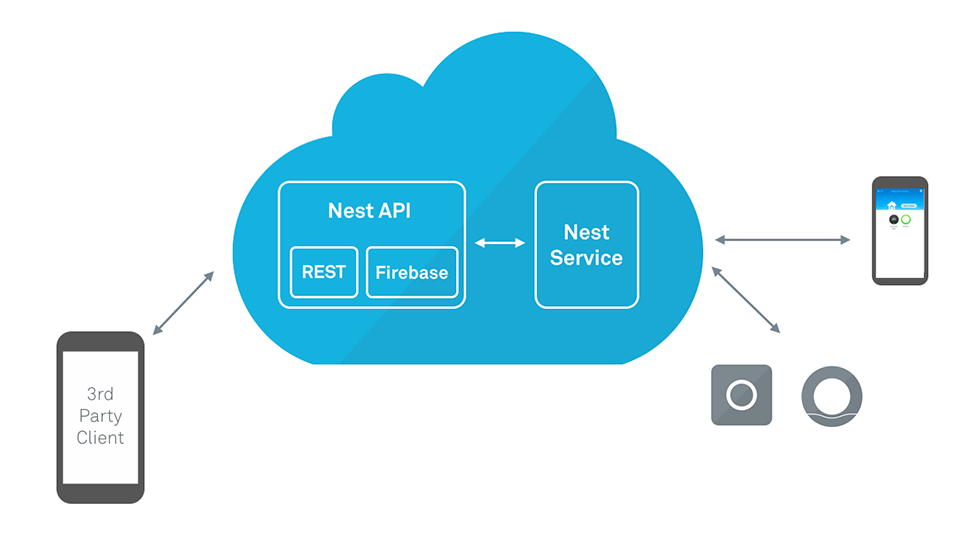
\includegraphics[width=8cm]{pics/howitworks}
\eit

\subsection{Example}
\bit
\w Client for the \bb{Nest Learning Thermostat} that monitors two values:
\textcolor{blue2}{current temperature} and \textcolor{blue2}{target
  temperature}

\w When your customer (i.e. human) adjusts the temperature at the Nest
Thermostat, the \textcolor{blue2}{target temperature} changes and the Nest
service updates the JSON doc, which is synchronized in real time 

\w Your client \textcolor{red2}{\bb{listens for}} (HOW?) changes, then:

  \bit
  \w displays the new target temperature
  \w updates the current temperature as it changes
  \eit

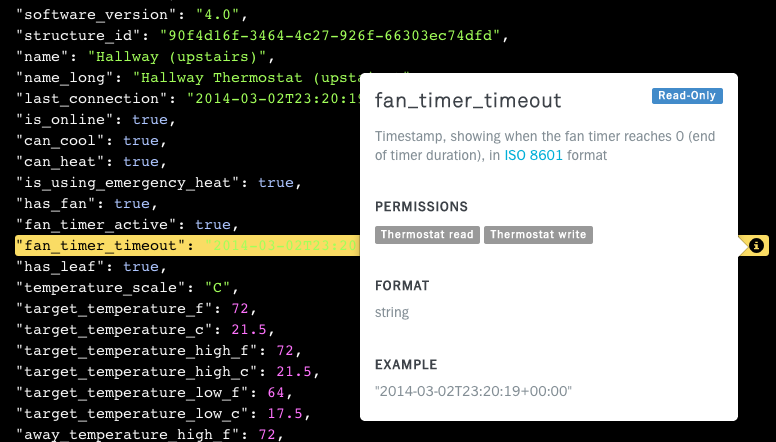
\includegraphics[width=8cm]{pics/api-viewer}
\eit


\begin{figure*}
\small\tt
\centerline{\begin{tabular}{|l|l|l|}\hline
\multicolumn{1}{|c}{structures} & \multicolumn{2}{|c|}{devices} \\ \hline
 & thermostats & smoke\_co\_alarms \\ \hline
    structure\_id & device\_id & device\_id \\
    thermostats & locale & locale \\
    smoke\_co\_alarms & software\_version & software\_version \\ 
    away &     structure\_id &     structure\_id \\
    name & name & name \\
    country\_code & name\_long & name\_long \\
    peak\_period\_start\_time & last\_connection & last\_connection \\
    peak\_period\_end\_time & is\_online & is\_online \\
    time\_zone & can\_cool & battery\_health \\
    eta & can\_heat & co\_alarm\_state \\
     & can\_heat & smoke\_alarm\_state \\
     & is\_using\_emergency\_heat & ui\_color\_state \\
    & has\_fan & \\
    & fan\_timer\_active & \\
    & fan\_timer\_timeout & \\
    & has\_leaf & \\
    & temperature\_scale & \\
    & target\_temperature & \\
    & target\_temperature\_high & \\
    & target\_temperature\_low & \\
    & away\_temperature\_high & \\
    & away\_temperature\_low & \\
    & hvac\_mode & \\
    & ambient\_temperature & \\ \hline
  \end{tabular}}
  \rm\small
  \caption{Current Nest data model -- not sure how to extend this (e.g. add
    new field)}
\end{figure*}

\section{Authentication and authorization}
\subsection{Three per-structure permissions}
\bit
\w \bb{Away read}:
  grants read permission to most of the Structure data values
\w \bb{Away read/write}:
   \bit  
   \w grants read permission to most of the Structure data values
   \w grants read/write permission for \textcolor{red2}{\bf{}away}
   \eit
\w \bb{ETA write}
   \bit
   \w  grants read permission to most of the Structure data values
   \w grants write permission for \textcolor{red2}{\bf{}away}

   \eit
\eit

\subsection{Two per-thermostat permissions}
\bit
\w \bb{Thermostat read}
   \bit
   \w Grants read permission to most of the Thermostat and Structure data
   values
   \eit
\w \bb{Thermostat read/write}
  \bit
  \w Grants read permission to all of the Thermostat data values
  \w Grants write permission to these Thermostat data values:
        \textcolor{red2}{\texttt{is\_fan\_timer\_active}}, all 
        \textcolor{red2}{\texttt{target\_temperature\ fields}} and 
        \textcolor{red2}{\texttt{hvac\_mode}}
 \w Grants read permission to most of the \bb{Structure} data values
  \eit
\eit


\section{REST and REST Streaming Interfaces}
\subsection{REST Streaming}
In addition to the standard REST interface, the Nest service also supports
REST Streaming. You may want to use REST if your preferred development
environment or programming language has no compatible helper library and does
not support \textcolor{blue2}{\bf{}WebSockets}. If your client needs to
  receive real time updates from the Nest service via REST, then you'll want
  to use REST Streaming.  

Like the standard REST interface, Nest's REST Streaming implementation is
based on Firebase. You can learn more about REST Streaming on the Firebase web
site. As you read through the Firebase REST Streaming reference, keep in mind
these differences with Nest's implementation: 
\bit
\w \textcolor{red2}{\texttt{cancel}} event is not supported
\w \textcolor{red2}{\texttt{patch}} event is not supported
\w     Your REST clients will need to handle redirects with status code 307
\w     Data rate limiting may be applied to your clients
\eit

\paragraph{REST Streaming and rate limits}
In order to prevent overutilization of the Nest service, we limit the number of connections a client can make in a specific time period. If you're using the Firebase client you shouldn't hit these limits, as a single connection can handle all communication over a long period of time. For REST Streaming calls, each access token has a limited number of read calls.

\paragraph{REST Streaming and redirects}
Another consideration of using REST Streaming is that your client must also handle 307 redirects.


\end{document}
